\documentclass[a4paper,12pt]{article} % тип документа
\usepackage[margin=1in]{geometry} % Поля

%  Русский язык
\usepackage[warn]{mathtext}
\usepackage[T2A]{fontenc}			% кодировка
\usepackage[utf8]{inputenc}			% кодировка исходного текста
\usepackage[english,russian]{babel}	% локализация и переносы
% Математика
\usepackage{amsmath,amsfonts,amssymb,amsthm,mathtools} 
\usepackage{wasysym}
%%%
\usepackage{graphicx}

\usepackage{tabularx}

\usepackage{gensymb} % знак градуса
\usepackage{enumitem} % изменить список enumerate
\usepackage{placeins} % \FloatBarrier

\renewcommand{\thesection}{\Roman{section}} 
\renewcommand{\thesubsection}{\roman{subsection}}


\begin{document}

\newcolumntype{Y}{>{\centering\arraybackslash}X} %new tabularx


%титул
\hrule 	
\medskip
\begin{raggedright}
{\large \textbf{Отчёт по работе 4.3.1}}
\\
\medskip
{\Large Изучение дифракции света} 
\\
\medskip
{\large Карташов Констанин Б04-005}
\medskip
\hrule
\medskip
\end{raggedright}


\section{Анотация}

\paragraph{Цель работы:} 
Исследовать явления дифракции Френеля и Фраунгофера на щели, изучить влияние дифракции на разрешающую способность оптических инструментов.

\paragraph{Оборудование:}
\begin{itemize}
\renewcommand{\labelitemi}{$\triangleright$}
\itemsep-0.5em
\item оптическая скамья,
\item ртутная лампа,
\item монохроматор, 
\item щели с регулируемой шириной с микрометрическим винтом,
\item рамка с вертикальной нитью,
\item двойная щель,
\item микроскоп на поперечных салазках,
\item зрительная труба.
\end{itemize}


\medskip\hrule\medskip

\section{Теоретическая часть}

\paragraph{} Дифракцией, в широком смысле, называют отклонение в распространении волн от законов геометрической оптики. Для определения вида дифракционной картины можно ввести волновой параметр:

\[
p = \frac{\sqrt{\lambda z}}{b},
\]

\noindent где $\lambda$ -- длинная падающей волны, $z$ -- расстояние до отверстия, $b$ -- характеристический размер отверстия. В случае когда $p \ll 1$ для описания света справедливы законы геометрической оптики, при $p \sim 1$ -- происходит дифракция Френеля, при $p \gg 1$ --  дифракция Фраунгофера.


\medskip\hrule\medskip

\section{Экспериментальная часть}

\subsection{Дифракция Френеля на щели}

\begin{figure}[h]
\centering
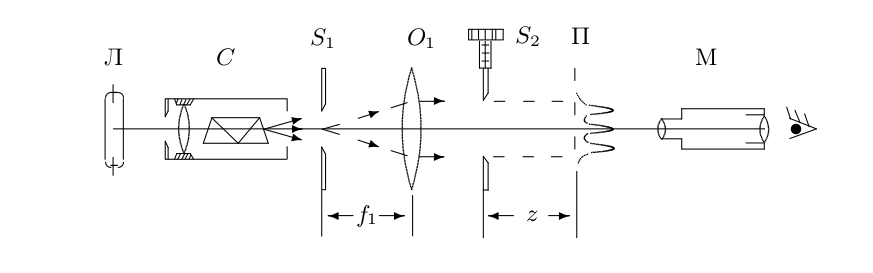
\includegraphics[width=\textwidth]{setup1.png}
\caption{Схема установки для изучения дифракции Френеля на щели}
\label{fig:setup1}
\end{figure}

\paragraph{} Соберём экспериментальную установку в на оптической скамье в соответствии с рис. \ref{fig:setup1} (вместо монохроматора используем светофильтр). 

Найдём начальное положение микрометрическое винта на щели $S_2$, медленно открывая её вращением винта, после нескольких измерений получаем начальное значение $b_0 = 38 \div 42 = 40 \pm 2$ мкм.

В объективе микроскопа получим резкое изображение щели. Отметим начала отчёта $z_0 = 45.1$ см. Далее, передвигая микроскоп, запишем положения при которых чётко видны чёрные полосы, и количество чёрных полос.

По микрометрическому винту измерим размер щели: $b_\text{винт} = 340 \pm 5$ мкм, с учётом начального положения винта и его погрешности: $b_\text{винт} = 300 \pm 5$ мкм. Теперь измерим ширину при помощи микроскопа: $b_\text{микр} = 320 \pm 10$ мкм.

Количество видимых чёрных линий связано на один меньше, чем количество видимых зон Френеля.

Данные измерений приведены в таблице \ref{tab:exp1}.

\begin{table}[h]
\centering
\begin{tabular}{|l|l|l|l|}
\hline
$n_\text{полос}$ & $z$, см & $z_\text{отн}$, см & $m_\text{зон Френеля}$ \\ \hline
1                & 42.5    & 2.6                & 2                      \\ \hline
2                & 43.4    & 1.7                & 3                      \\ \hline
3                & 43.8    & 1.3                & 4                      \\ \hline
4                & 44.1    & 1.0                & 5                      \\ \hline
5                & 44.3    & 0.8                & 6                      \\ \hline
\end{tabular}
\caption{Данные измерений}
\label{tab:exp1}
\end{table}

\paragraph{} Построим график зависимости $z(m)$ по данным из табл. \ref{tab:exp1} (рис. \ref{fig:exp2}). Теоретическая зависимость $z(m)$ имеет вид:

\[
z = \frac{b^2}{4\lambda} \frac{1}{m},
\]

\noindent где $b$ -- ширина щели, $\lambda$ -- длина волны падающего света. Пользуясь методом наименьших квадратов для функции вида $y = a/x$ найдём наилучшею кривую и случайную погрешность. Получаем:

\[ 
a = \frac{b^2}{4 \lambda} = 5.14 \text{ см} \; \Rightarrow \; b = 2\sqrt{5.14 \text{ см} \cdot \lambda} = 2 \sqrt{5.14 \text{ см} \cdot 578.2 \text{ нм}} = 345 \text{ мкм},
\]\[
\sigma_b = b \cdot \frac{\sigma_a}{2a} = 2 \text{ мкм}.
\]

\noindent Получаем $b = 345 \pm 2$ мкм.

\begin{figure}
\centering
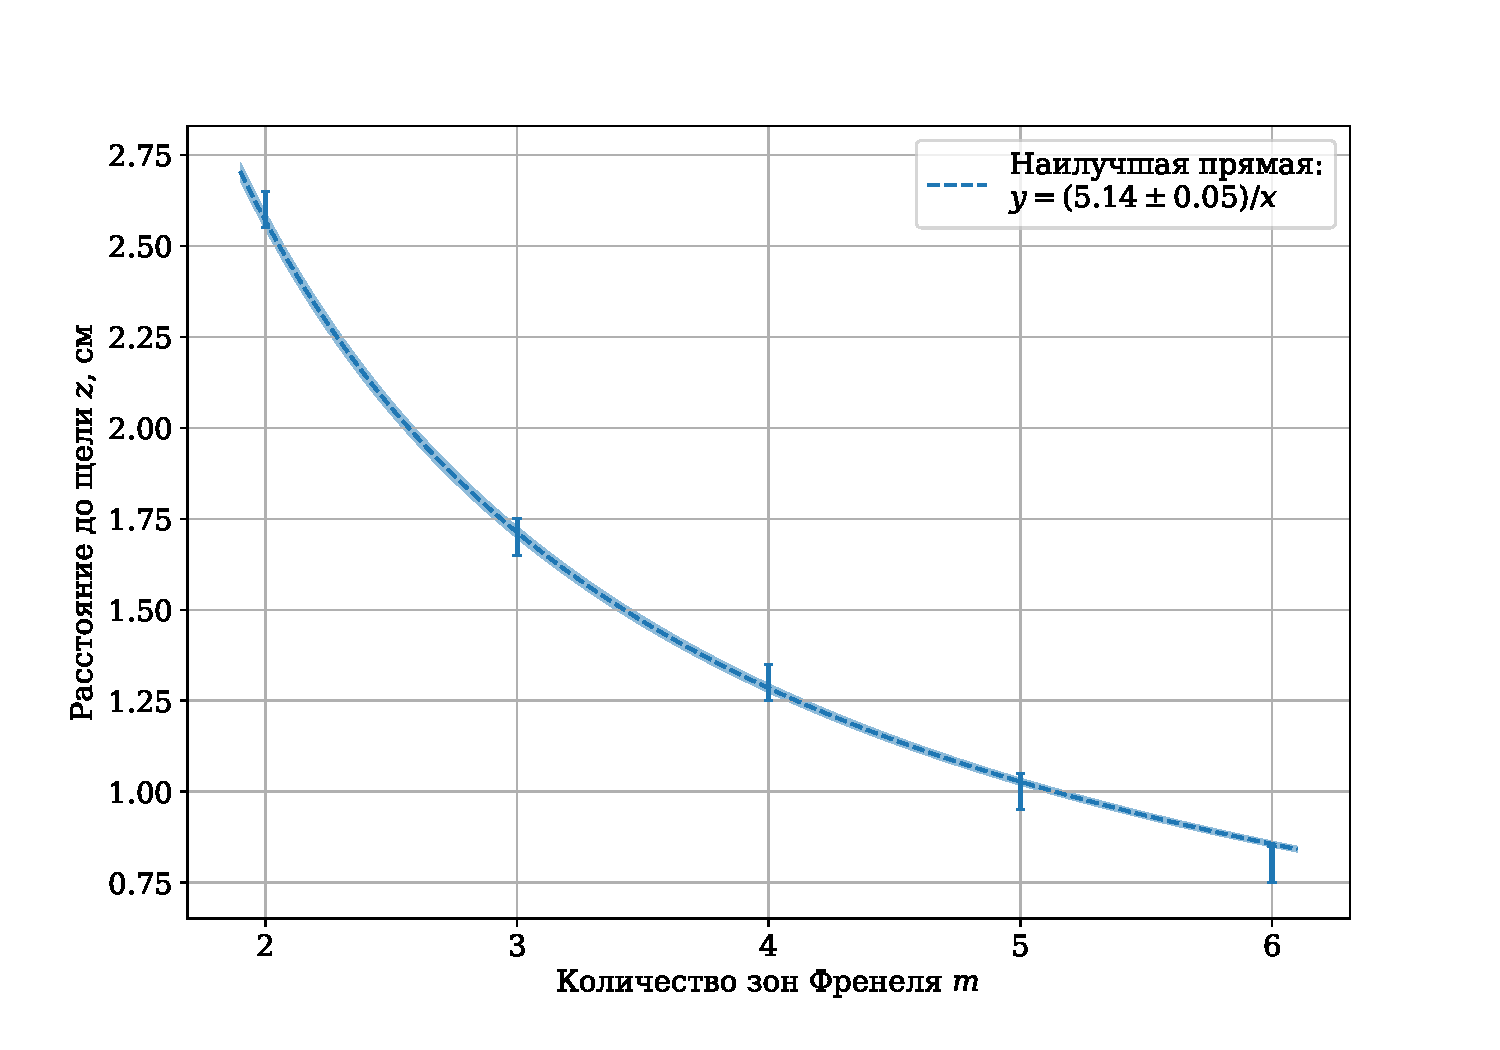
\includegraphics[width=\textwidth]{exp1.pdf}
\caption{График зависимости $z(m)$ с наилучшей кривой}
\label{fig:exp1}
\end{figure}

\paragraph{} Пронаблюдаем дифракцию на краю Экрана, слегка отодвинув микроскоп от положения в котором чётко видно щель. Видим, что у краёв щели появились частые узкие полосы. Возле краёв щели расположена самая яркая светлая полоса, она соответствует первому полу-витку спирали Корню.

\paragraph{} Начнём уменьшать размер щели, наблюдая за изменением дифракционной картины. Видим, что число тёмных полос уменьшается, при этом их толщина почти не изменяется.

\paragraph{} Пронаблюдаем дифракцию Френеля на тонкой проволоке. Видим, что центр проволоки остаётся светлым, а количество тёмных полос всегда чётно.

\subsection{Дифракция Фраунгофера на щели}

\begin{figure}[h]
\centering
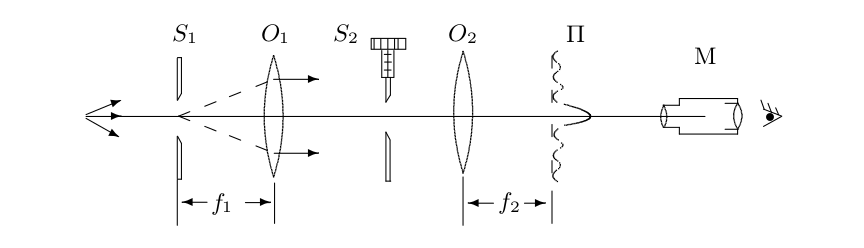
\includegraphics[width=\textwidth]{setup2.png}
\caption{Схема установки для изучения дифракции Фраунгофера на щели}
\label{fig:setup2}
\end{figure}

\paragraph{} Соберём экспериментальную установку на оптической скамье согласно рис. \ref{fig:setup2}. Размер щели $b = 360 \pm 5$ мкм. Фокусное расстояние второй линзы $f_2 = 15.5$ см.

Измерим положения нескольких поперечных минимумов табл. \ref{tab:exp2}. По измеренным данным построим график и проведём наилучшею прямую пользуясь методом наименьших квадратов. Найдём среднее расстояние между минимумами с учётом случайной погрешности. Получаем $\Delta x = 0.234 \pm 0.002$ мм.

\begin{table}[h]
\centering
\begin{tabular}{|l|l|l|l|l|l|l|l|l|}
\hline
$m$     & $+1$ & $-1$ & $+2$ & $-2$ & $+3$ & $-3$ & $+4$ & $-4$ \\ \hline
$x$, мм & 2.24 & 1.74 & 2.48 & 1.54 & 2.72 & 1.28 & 2.92 & 1.08 \\ \hline
\end{tabular}
\caption{Положения максимумов и минимумов}
\label{tab:exp2}
\end{table}


\begin{figure}
\centering
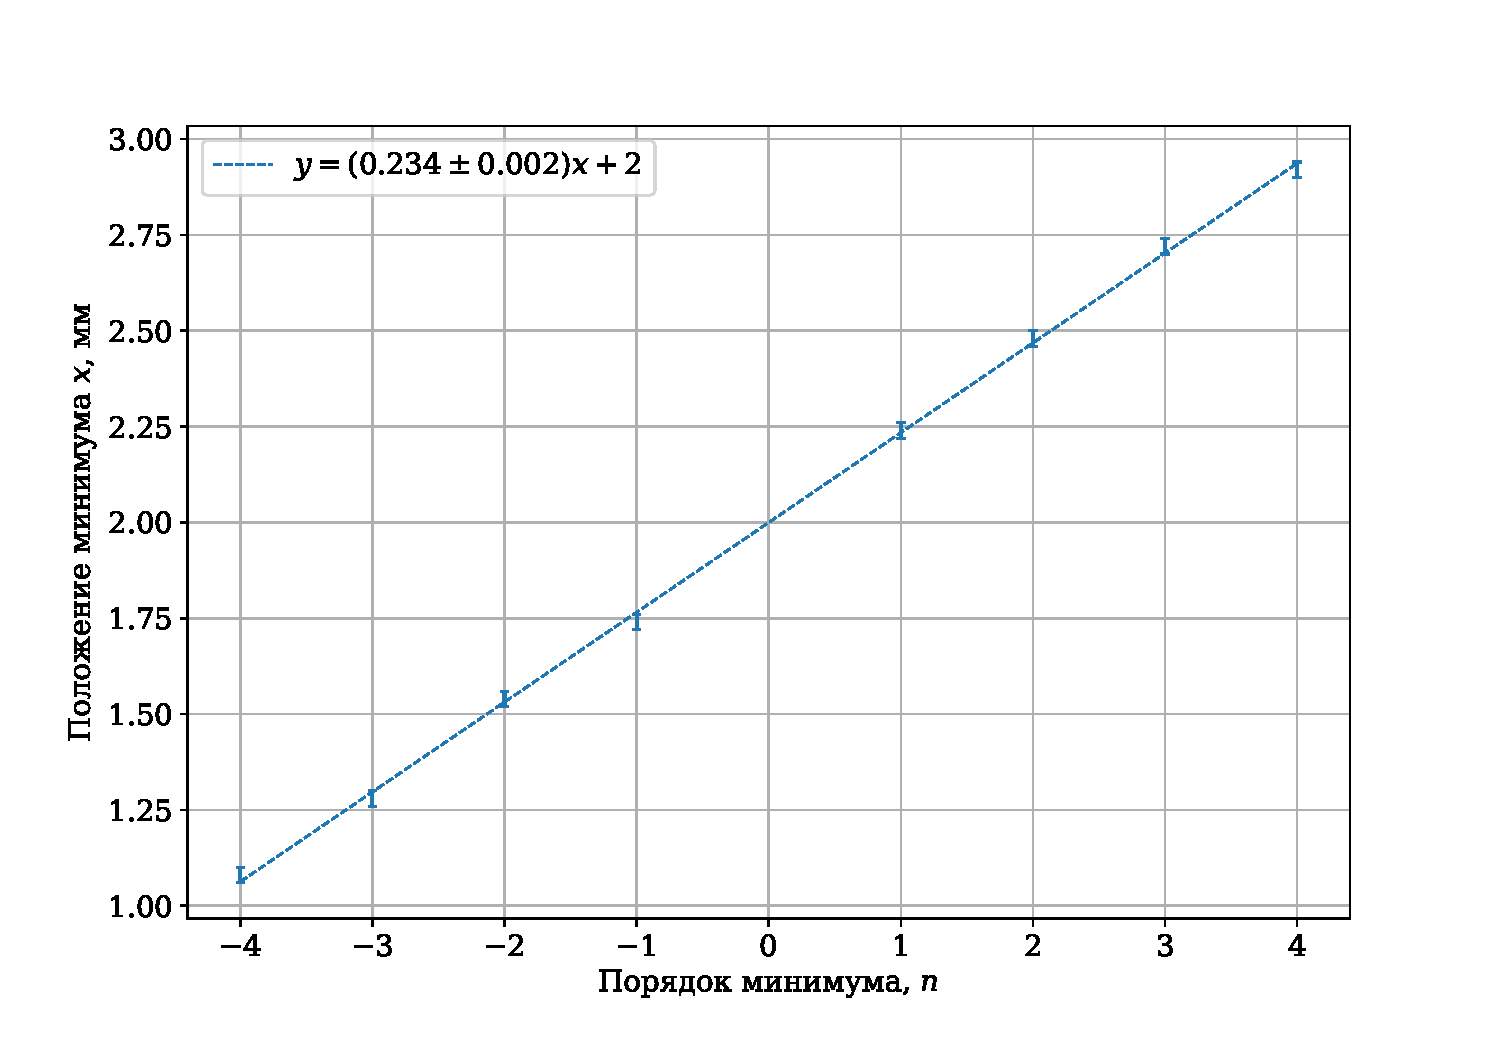
\includegraphics[width=\textwidth]{exp2.pdf}
\caption{График положений минимумов с проведённой наилучшей прямой.}
\label{fig:exp2}
\end{figure}

\paragraph{} Рассчитаем размер щели пользуясь формулой:

\[
x_m = m \frac{\lambda}{b} f_2 \; \Rightarrow \; \Delta x = \frac{\lambda}{b} f_2 \; \Rightarrow \; b = \frac{\lambda f_2}{\Delta x}.
\]

\noindent Получаем:

\[
b = \frac{578.2 \text{ нм} \cdot 15.5 \text{ см}}{0.234 \text{ мм}} = 383 \text{ мкм},
\]\[
\sigma_b = b \frac{\sigma_{\Delta x}}{\Delta x} = 3 \text{ мкм}.
\]

\noindent Получаем $b = 383 \pm 3$ мкм.

\paragraph{} Переместим щель $S_2$ в боковом направлении. Видим, что при этом дифракционная картина не перемещается, но при дальнейшем смещении щели, дифракционная картина становится менее чётком, и различимо меньшее количество максимумов.

\paragraph{} Уменьшим размер щели $S_2$. Видим, что масштаб дифракционной картины увеличился.


\subsection{Дифракция Фраунгофера на двух щелях}

\begin{figure}[h]
\centering
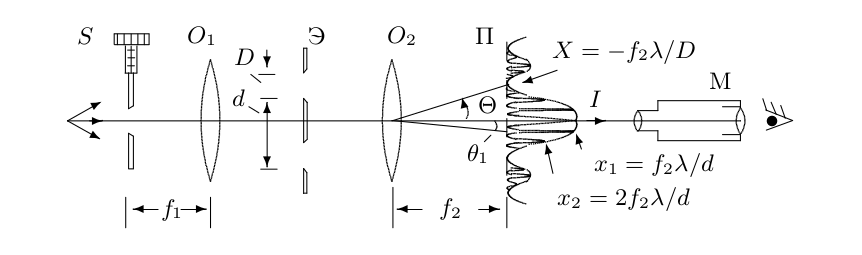
\includegraphics[width=\textwidth]{setup3.png}
\caption{Схема установки для изучения дифракции Фраунгофера на двух щелях}
\label{fig:setup3}
\end{figure}

\paragraph{} Соберём экспериментальную установку на оптической скамье согласно рис. \ref{fig:setup3}. Фокусное расстояние первой и второй линзы соответственно $f_1 = 11.0$ см и $f_2 = 15.5$ см.

\paragraph{} При помощи микроскопа измерим размеры щелей расстояние между ними. Измеренные координаты четырёх вертикалей: $x_1 = 1.00$ мм, $x_2 = 1.18$ мм, $x_3 = 1.82$ мм, $x_4 = 1.98$ мм. Получаем размер щелей $b = 0.17 \pm 0.02$ мм, расстояние между щелями $d = 0.81 \pm 0.02$ мм.

\paragraph{} Получим в окуляре микроскопа чёткое изображение дифракционной картины. Посчитаем координаты самых удалённых друг от друга тёмных полос в центральном максимуме: $x_1 = 1.48 \pm 0.01$ мм, $x_2 = 2.50 \pm 0.01$ мм и число светлых промежутков между ними: $N = 17$. Размер центрального максимума $\Delta x = x_2 - x_1 = 1.02 \pm 0.02$ мм. 

Посчитаем расстояние между минимумами $\delta x = \Delta x / N = 0.060 \pm 0.001$ мм $ = 60 \pm 1$ мкм. Рассчитаем расстояние между щелями $d$ по формуле:

\[
\delta x = f_2 \frac{\lambda}{d} \; \Rightarrow \; d = \frac{f_2 \lambda}{\delta x} = \frac{15.5 \text{ см} \cdot 578.2 \text{ нм}}{60 \text{ мкм}} = 1.49 \pm 0.02 \text{ мм}.
\]

Рассчитаем число полос в центральном максимуме по формуле:

\[
n = \frac{2 \lambda f_2}{b} \frac{1}{\delta x} = \frac{2d}{b} = \frac{2 \cdot 0.81}{0.17} \approx 10.
\]

\paragraph{} Будем менять размер щели пока дифракционная картина не станет размыто	й. Получаем размеры щели $b = 44 \div 47$ мкм. Это должно произойти при равенстве размера щели с радиусом когерентности щели:

\[
d = \frac{\lambda f_1}{b_0} \; \Rightarrow \; b_0 = \frac{\lambda f_1}{d} =  \frac{578.2 \text{ нм} \cdot 11 \text{ см}}{0.8 \text{ мм}} = 80 \text{ мкм}.
\]

\noindent Рассчитанное значение близко к реальному.

\subsection{Влияние дифракции на разрешающую способность оптического прибора}

\begin{figure}[h]
\centering
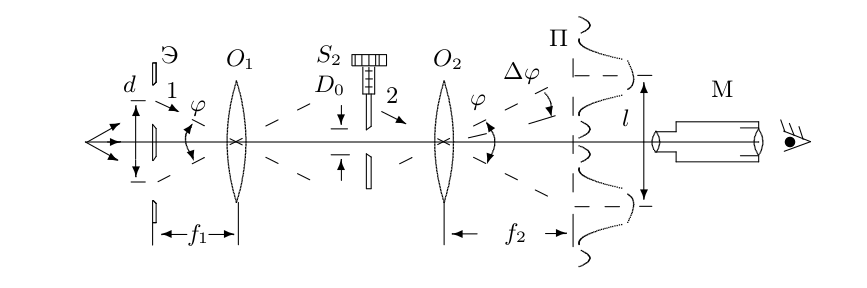
\includegraphics[width=\textwidth]{setup4.png}
\caption{\centering Схема установки для изучения влияния дифракции на разрешающую способность  оптического прибора}
\label{fig:setup4}
\end{figure}

\paragraph{} Соберём экспериментальную установку на оптической скамье согласно рис. \ref{fig:setup4}. Линзы и пластинка с двойной щелью такие же как на прошлой установке.

\paragraph{} В окуляре микроскопа получим чёткое изображение двух щелей. Меняя размер щели $S_2$ пронаблюдаем за тем как изменяется чёткость изображения. При уменьшении размеров щели изображение становится более размытым. Минимальный размер щели при котором различимы две отдельные щели $b_0 \approx 45$ мкм. Видим, что это значение совпадает со значением при котором размывается дифракционная картина в прошлом пункте. Сравним это с минимальным расстоянием рассчитанным по критерию Рэлея:

\[
\delta x \sim l \; \Rightarrow \; \frac{\lambda}{b} \sim \frac{d}{f_1} \; \Rightarrow \; b_0 \sim \frac{\lambda f_1}{d} = \frac{578.2 \text{ нм} \cdot 11 \text{ см}}{0.8 \text{ мм}} = 80 \text{ мкм}. 
\]

\medskip\hrule\medskip

\section{Выводы}

\begin{enumerate}
\item Пронаблюдали дифракцию Френеля для щели и проволоки. Найдя положения в которых чётко виды тёмные полосы, нашли положения в которых видно целое число зон Френеля. Исходя из этого вычислили размер щели. Получили размеры щели посчитанные несколькими способами: микрометрическим винтом $b_\text{винт} = 300 \pm 5$ мкм, микроскопом $b_\text{микро} = 320 \pm 10$, по зонами Френеля $b = 345 \pm 2$ мкм.

\item Пронаблюдали дифракцию Фраунгофера на щели. Посчитав расстояние между минимумами, вычислим размер щели $b = 383 \pm 3$ мкм, размер измеренные микрометрическим винтом $b_\text{винт} = 360 \pm 5$ мкм. Убедились в том, что сдвиг щели не влияет на размеры интерференционной картины.

\item Пронаблюдали дифракцию Фраунгофера на двух щелях. По наблюдениям рассчитали расстояние между щелями $d = 1.49 \pm 0.02$ мм, расстояние измеренное микроскопом $d_\text{микро} = 0.81 \pm 0.02$. Нашли положение, в котором интерференционная картина размыта $b_0 \approx 45$ мкм. Сравним с предельными размером щели из соображений когерентности $b_\text{ког} \approx 80$ мкм.

\item Пронаблюдаем изображение двух щелей в микроскоп. Меняя размер щели-объектива микроскопа найдём размер щели при котором изображение двух щелей перестаёт быть различимым $b_0 \approx 45$ мкм. Рассчитаем это значение из критерия Рэлея $b_\text{Релей} \approx 80$ мкм. Видим, что значение получились такие же, как при наблюдении дифракции Фраунгофера на двух щелях.


\end{enumerate}


\medskip\hrule\medskip

\end{document}
